\documentclass[10pt]{article}
\usepackage[utf8]{inputenc}
\usepackage[T1]{fontenc}
\usepackage{amsmath}
\usepackage{amsfonts}
\usepackage{amssymb}
\usepackage[version=4]{mhchem}
\usepackage{stmaryrd}
\usepackage{graphicx}
\usepackage[export]{adjustbox}
\graphicspath{ {./images/} }
\usepackage{bbold}

\begin{document}
\section*{Math 141 Tutorial 6 Solutions}
\section*{Main problems}
\begin{enumerate}
  \item Compute the following using trigonometric substitution.\\
(a) $\int t^{3}\left(3 t^{2}-4\right)^{5 / 2} \mathrm{~d} t$\\
(c) $\int \frac{1}{\sqrt{9 x^{2}-36 x+37}} \mathrm{~d} x$\\
(b) $\int \frac{\sqrt{x^{2}+16}}{x^{4}} \mathrm{~d} x$\\
(d) $\int \frac{(x+3)^{5}}{\left(40-6 x-x^{2}\right)^{3 / 2}} \mathrm{~d} x$
\end{enumerate}

Solution:\\
(a) The trigonometric substitution we will use is:\\
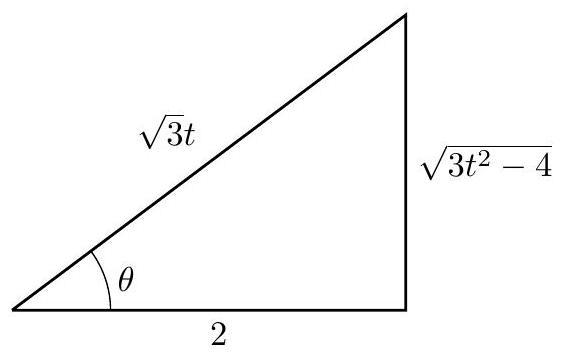
\includegraphics[max width=\textwidth, center]{2024_12_27_cdb9098edf96ee128a6eg-01}

$$
\begin{aligned}
& 2 \sec \theta=\sqrt{3} t \\
& 2 \sec \theta \tan \theta \mathrm{~d} \theta=\sqrt{4} t \mathrm{~d} t \\
& \tan \theta=\frac{\sqrt{3 t^{2}-4}}{2}
\end{aligned}
$$

With this, we have

$$
\begin{aligned}
\int t^{3}\left(3 t^{2}-4\right)^{5 / 2} \mathrm{~d} t & =\int \frac{2^{3} \sec ^{3} \theta}{3^{3 / 2}}\left(4 \sec ^{2} \theta-4\right)^{5 / 2} \frac{2 \sec \theta \tan \theta}{\sqrt{3}} \mathrm{~d} \theta \\
& =\frac{512}{9} \int \sec ^{4} \theta \tan ^{6} \theta \mathrm{~d} \theta \\
& =\frac{512}{9} \int \sec ^{2} \theta\left(1+\tan ^{2} \theta\right) \tan ^{6} \theta \mathrm{~d} \theta
\end{aligned}
$$

Using the substitution $u=\tan \theta$, we get $\mathrm{d} u=\sec ^{2} \theta \mathrm{~d} \theta$ and hence

$$
\begin{aligned}
\int t^{3}\left(3 t^{2}-4\right)^{5 / 2} \mathrm{~d} t & =\frac{512}{9} \int \sec ^{2} \theta\left(1+\tan ^{2} \theta\right) \tan ^{6} \theta \mathrm{~d} \theta \\
& =\frac{512}{9} \int\left(1+u^{2}\right) u^{6} \mathrm{~d} u \\
& =\frac{512}{9}\left(\frac{u^{7}}{7}+\frac{u^{9}}{9}\right)+C \\
& =\frac{512}{9}\left(\frac{\tan ^{7} \theta}{7}+\frac{\tan ^{9} \theta}{9}\right)+C \\
& =\frac{512}{9}\left(\frac{1}{7}\left(\frac{\sqrt{3 t^{2}-4}}{2}\right)^{7}+\frac{1}{9}\left(\frac{\sqrt{2 t^{2}-4}}{2}\right)^{9}\right)+C \\
& =\frac{4\left(3 t^{2}-4\right)^{7 / 2}}{63}+\frac{\left(3 t^{2}-4\right)^{9 / 2}}{81}+C
\end{aligned}
$$

(b) The trigonometric substitution we will use is:\\
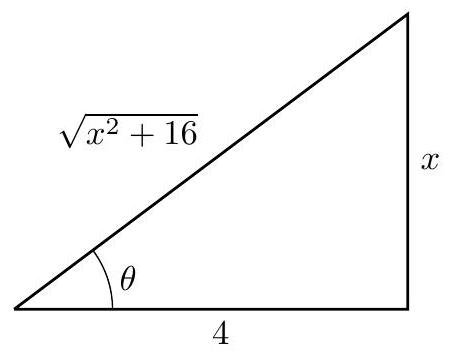
\includegraphics[max width=\textwidth, center]{2024_12_27_cdb9098edf96ee128a6eg-02}

$$
\begin{aligned}
& 4 \tan \theta=x \\
& 4 \sec ^{2} \theta \theta=\mathrm{d} x \\
& \sin \theta=\frac{x}{\sqrt{x^{2}+16}}
\end{aligned}
$$

With this, we have

$$
\begin{aligned}
\int \frac{\sqrt{x^{2}+16}}{x^{4}} \mathrm{~d} x & =\int \frac{\sqrt{16 \tan ^{2} \theta+16}}{64 \tan ^{4} \theta} 4 \sec ^{2} \theta \mathrm{~d} \theta \\
& =\frac{1}{16} \int \frac{\sec ^{3} \theta}{\tan ^{4} \theta} \mathrm{~d} \theta \\
& =\frac{1}{16} \int \frac{1}{\cos ^{3} \theta} \frac{\cos ^{4} \theta}{\sin ^{4} \theta} \mathrm{~d} \theta \\
& =\frac{1}{16} \int \frac{\cos \theta}{\sin ^{4} \theta} \mathrm{~d} \theta
\end{aligned}
$$

Page 2

Using the substitution $u=\sin \theta$, we get $\mathrm{d} u=\cos \theta \mathrm{d} \theta$ and hence

$$
\begin{aligned}
\int \frac{\sqrt{x^{2}+16}}{x^{4}} \mathrm{~d} x & =\frac{1}{16} \int \frac{\cos \theta}{\sin ^{4} \theta} \mathrm{~d} \theta \\
& =\frac{1}{16} \int u^{-4} \mathrm{~d} u \\
& =\frac{-1}{48 u^{3}}+C \\
& =\frac{-1}{48 \sin ^{3} \theta}+C \\
& =\frac{-\left(x^{2}+16\right)^{3 / 2}}{48 x^{3}}
\end{aligned}
$$

(c) Completing the square in the square root gives

$$
9 x^{2}-36 x+37=(3 x-6)^{2}-1
$$

Thus the trigonometric substitution we will use is:\\
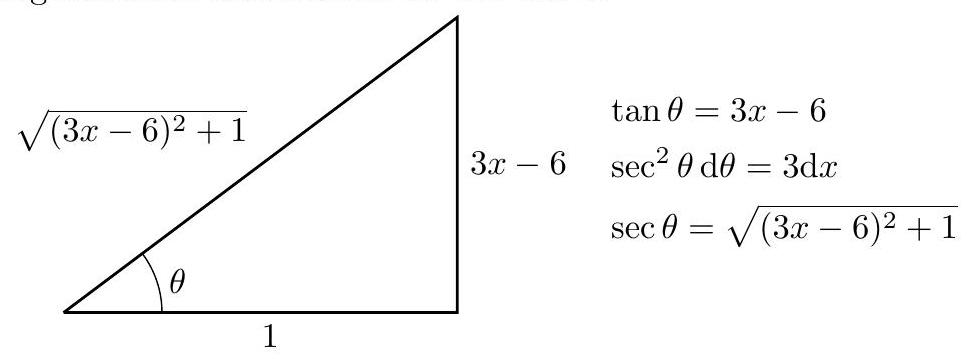
\includegraphics[max width=\textwidth, center]{2024_12_27_cdb9098edf96ee128a6eg-03}

With this, we have

$$
\begin{aligned}
\int \frac{1}{\sqrt{(3 x-6)^{2}+1}} \mathrm{~d} x & =\int \frac{\sec ^{2} \theta \mathrm{~d} \theta}{3 \sqrt{\tan ^{2} \theta+1}} \\
& =\frac{1}{3} \int \frac{\sec ^{2} \theta}{\sec \theta} \mathrm{~d} \theta \\
& =\frac{1}{3} \int \sec \theta \mathrm{~d} \theta \\
& =\frac{1}{3} \ln \left|\sqrt{\left(3 x^{2}-6\right)^{2}+1}+3 x-6\right|+C .
\end{aligned}
$$

(d) Completing the square in the square root gives

$$
40-6 x-x^{2}=49-(x+3)^{2}
$$

Thus the trigonometric substitution we will use is:\\
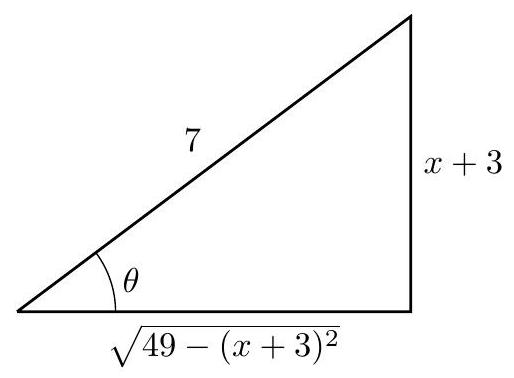
\includegraphics[max width=\textwidth, center]{2024_12_27_cdb9098edf96ee128a6eg-04}

$$
\begin{aligned}
& \sin \theta=x+3 \\
& 7 \cos \theta \mathrm{~d} \theta=\mathrm{d} x \\
& \cos \theta=\frac{\sqrt{49-(x+3)^{2}}}{7}
\end{aligned}
$$

With this, we have

$$
\begin{aligned}
\int \frac{(x+3)^{5}}{\left(49-(x+3)^{2}\right)^{3 / 2}} \mathrm{~d} x & =\int \frac{7^{5} \sin ^{5} \theta}{\left(49-49 \sin ^{2} \theta\right)^{3 / 2}} 7 \cos \theta \mathrm{~d} \theta \\
& =343 \int \frac{\sin ^{5} \theta}{\cos ^{2} \theta} \mathrm{~d} \theta \\
& =343 \int \frac{\left(1-\cos ^{2} \theta\right)^{2}}{\cos ^{2} \theta} \sin \theta \mathrm{~d} \theta .
\end{aligned}
$$

Using the substitution $u=\cos \theta$, we get $\mathrm{d} u=-\sin \theta \mathrm{d} \theta$ and hence

$$
\begin{aligned}
\int \frac{(x+3)^{5}}{\left(49-(x+3)^{2}\right)^{3 / 2}} \mathrm{~d} x & =343 \int \frac{\left(1-\cos ^{2} \theta\right)^{2}}{\cos ^{2} \theta} \sin \theta \mathrm{~d} \theta \\
& =-343 \int \frac{\left(1-u^{2}\right)^{2}}{u^{2}} \mathrm{~d} \theta \\
& =-343 \int \frac{1-u^{2}+u^{4}}{u^{2}} \mathrm{~d} u \\
& =-343 \int u^{-2}-2+u^{2} \mathrm{~d} u \\
& =-343\left(\frac{-1}{u}-2 u+\frac{u^{3}}{3}\right)+C \\
& =-343\left(\frac{-1}{\cos \theta}-\cos \theta+\frac{\cos ^{3} \theta}{3}\right)+C, \\
& =343\left(\frac{7}{\sqrt{49-(x+3)^{2}}}+2 \frac{\sqrt{49-(x+3)^{2}}}{7}-\frac{\left(49-(x+3)^{2}\right)^{3 / 2}}{1029}\right)+C
\end{aligned}
$$

\begin{enumerate}
  \setcounter{enumi}{1}
  \item Use long division to express each of the following functions $f(x)$ as a proper fraction. That is, find polynomials $S(x), R(x), Q(x)$ such that
\end{enumerate}

$$
f(x)=S(x)+\frac{R(x)}{Q(x)}
$$

and $\operatorname{deg} R<\operatorname{deg} Q$.\\
(a) $f(x)=\frac{x^{2}+1}{x+1}$\\
(c) $f(x)=\frac{x^{3}+x^{2}-4 x+6}{x^{2}-2 x+2}$\\
(b) $f(x)=\frac{2 x^{3}-x}{x+3}$\\
(d) $f(x)=\frac{x^{4}+x+1}{\left(x^{2}+1\right)(x-1)}$

Solutions:\\
(a)

$$
\begin{aligned}
& \frac{-x^{2}-x}{-x+1} \\
& \frac{x+1}{2}
\end{aligned}
$$

Hence, $f(x)=x-1+\frac{2}{x+1}$\\
(b)

$$
\begin{aligned}
& 2 x^{2}-6 x+17 \\
& x+3) \quad 2 x^{3}-x \\
& -2 x^{3}-6 x^{2} \\
& -6 x^{2} \quad-x \\
& \frac{6 x^{2}+18 x}{17 x} \\
& \frac{-17 x-51}{-51}
\end{aligned}
$$

Hence, $f(x)=2 x^{2}-6 x+17-\frac{51}{x+3}$\\
(c)

$$
\begin{aligned}
& \left.x^{2}-2 x+2\right) \frac{x+3}{\frac{x^{3}+x^{2}-4 x+6}{}} \\
& \frac{-x^{3}+2 x^{2}-2 x}{3 x^{2}-6 x+6} \\
& \frac{-3 x^{2}+6 x-6}{0}
\end{aligned}
$$

Hence, $f(x)=x+3$\\
(d)

$$
\left.x^{3}-x^{2}+x-1\right) \begin{array}{r}
x+1 \\
\cline { 2 - 2 } \begin{array}{c}
x^{4} \\
-x^{4}+x^{3}-x^{2}+x \\
x^{3}-x^{2}+2 x+1 \\
-x^{3}+x^{2}-x+1 \\
x+2
\end{array}
\end{array}
$$

Hence, $f(x)=x+1+\frac{x+2}{\left(x^{2}+1\right)(x-1)}$\\
3. Write out the partial fraction decomposition for each of the following rational functions.\\
(a) $f(x)=\frac{1}{(x+a)(x+b)}$ when $a \neq b$\\
(c) $f(x)=\frac{x^{2}+x+1}{(x+1)^{2}(x+2)}$\\
(b) $f(z)=\frac{3 z^{2}-z+8}{z^{3}+4 z}$\\
(d) $f(t)=\frac{t^{2}+t+1}{t^{4}+2 t^{2}+1}$

Solutions:\\
(a) We have $f(x)=\frac{1}{(x+a)(x+b)}=\frac{A}{x+a}+\frac{B}{x+b}$. Multiplying by the denominator on either side, we obtain

$$
1=A(x+b)+B(x+a)=(A+B) x+(A b+B a)
$$

Hence $A+B=0$ or $B=-A$ and $A b+B a=1$. It follows that $a=A b+B a=A b-A a=$ $A(b-a)$ or $A=\frac{1}{b-a}$. This forces $B=-\frac{1}{b-a}=\frac{1}{a-b}$. In conclusion,

$$
f(x)=\frac{A}{x+a}+\frac{B}{x+b}=\frac{1}{(b-a)(x+a)}+\frac{1}{(a-b)(x+b)} .
$$

(b) We begin by factorizing the denominator: $z^{3}+4 z=\left(z^{2}+4\right) z$. Then, we write

$$
f(z)=\frac{3 z^{2}-z+8}{z^{3}+4 z}=\frac{A}{z}+\frac{B z+C}{z^{2}+4}
$$

Multiplying by the denominator on either side we see that

$$
3 z^{2}-z+8=A\left(z^{2}+4\right)+(B z+C) z=(A+B) z^{2}+C z+4 A
$$

Hence, $A+B=3, C=-1$ and $4 A=8$. This forces $A=2, B=1$ and $C=-1$. Therefore,

$$
f(z)=\frac{2}{z}+\frac{z-1}{z^{2}+4}
$$

(c) We have

$$
f(x)=\frac{x^{2}+x+1}{(x+1)^{2}(x+2)}=\frac{A}{x+1}+\frac{B}{(x+1)^{2}}+\frac{C}{x+2}
$$

Multiplying by the denominator on either side we find

$$
\begin{aligned}
x^{2}+x+1 & =A(x+1)(x+2)+B(x+2)+C(x+1)^{2} \\
& =(A+C) x^{2}+(3 A+B+2 C) x+(2 A+2 B+C)
\end{aligned}
$$

Hence

$$
\left\{\begin{aligned}
A+C & =1 \\
3 A+B+2 C & =1 \\
2 A+2 B+C & =1
\end{aligned}\right.
$$

We thus find $C=1-A$ and reduce the system to

$$
\left\{\begin{aligned}
A+B & =-1 \\
A+2 B & =0
\end{aligned}\right.
$$

This yields $A=-2 B$ so $-1=A+B=-2 B+B=-B$. Therefore, $B=1$. Working backwards, we find $A=-2$ and $C=1-A=3$. Ergo,

$$
f(x)=\frac{A}{x+1}+\frac{B}{(x+1)^{2}}+\frac{C}{x+2}=\frac{-2}{x+1}+\frac{1}{(x+1)^{2}}+\frac{3}{x+2} .
$$

(d) We first factor the denominator: $t^{4}+2 t^{2}+1=\left(t^{2}+1\right)^{2}$. Hence,

$$
f(t)=\frac{t^{2}+t+1}{t^{4}+2 t^{2}+1}=\frac{A t+B}{t^{2}+1}+\frac{C t+D}{\left(t^{2}+1\right)^{2}}
$$

Multiplying by the denominator on either side we see that

$$
t^{2}+t+1=(A t+B)\left(t^{2}+1\right)+C t+D=A t^{3}+B t^{2}+(A+C) t+(B+D)
$$

Hence $A=0, B=1, A+C=1$ and $B+D=1$. This yields $C=1$ and $D=0$. Therefore

$$
f(t)=\frac{A t+B}{t^{2}+1}+\frac{C t+D}{\left(t^{2}+1\right)^{2}}=\frac{1}{t^{2}+1}+\frac{t}{\left(t^{2}+1\right)^{2}}
$$

\begin{enumerate}
  \setcounter{enumi}{3}
  \item Integrate the following rational functions.\\
(a) $\int_{0}^{1 / 2} \frac{1}{1-x^{2}} \mathrm{~d} x$\\
(d) $\int \frac{x^{4}+x+1}{\left(x^{2}+1\right)(x-1)} \mathrm{d} x$\\
(b) $\int \frac{1}{x^{2}(x+1)^{2}} \mathrm{~d} x$\\
(e) $\int_{0}^{4} \frac{y-1}{y^{2}+4 y+3} \mathrm{~d} y$\\
(c) $\int \frac{1}{x^{3}+x^{2}-x-1} \mathrm{~d} x$\\
(f) $\int_{2}^{4} \frac{t+1}{t^{3}-t^{2}} \mathrm{~d} t$
\end{enumerate}

Solutions:\\
(a) We use the method of partial fractions:

$$
\frac{1}{1-x^{2}}=\frac{1}{(1-x)(1+x)}=\frac{A}{1-x}+\frac{B}{1+x} .
$$

Multiplying by the denominator on either side by $1-x^{2}$ we see that

$$
1=A(1+x)+B(1-x)=(A-B) x+(A+B)
$$

Hence

$$
\left\{\begin{array}{l}
A-B=0 \\
A+B=1
\end{array}\right. \text {. }
$$

Solving, we find $A=B=1 / 2$. Thus, we obtain the partial fraction

$$
\frac{1}{1-x^{2}}=\frac{1 / 2}{1-x}+\frac{1 / 2}{1+x} .
$$

We can now evaluate the integral

$$
\begin{aligned}
\int_{0}^{1 / 2} \frac{1}{1-x^{2}} \mathrm{~d} x & =\int_{0}^{1 / 2} \frac{1 / 2}{1-x}+\frac{1 / 2}{1+x} \mathrm{~d} x \\
& =\frac{1}{2} \int_{0}^{1 / 2} \frac{1}{1-x} \frac{\mathrm{~d}}{\mathrm{~d} x}+\frac{1}{2} \int_{0}^{1 / 2} \frac{1}{1+x} \frac{\mathrm{~d}}{\mathrm{~d} x} \\
(y=1-x, z=1+x) & =-\frac{1}{2} \int_{1}^{1 / 2} \frac{1}{y} \frac{\mathrm{~d}}{\mathrm{~d} y}+\frac{1}{2} \int_{1}^{3 / 2} \frac{1}{z} \frac{\mathrm{~d}}{\mathrm{~d} z} \\
& =\frac{1}{2}\left(-\left.\ln (|y|)\right|_{y=1} ^{1 / 2}+\left.\ln (|z|)\right|_{z=1} ^{3 / 2}\right) \\
& =\frac{1}{2}[-\ln (1 / 2)+\ln (3 / 2)]=\frac{1}{2} \ln (3)
\end{aligned}
$$

(b) We write

$$
\frac{1}{x^{2}(x+1)^{2}}=\frac{A}{x}+\frac{B}{x^{2}}+\frac{C}{x+1}+\frac{D}{(x+1)^{2}} .
$$

Multiplying by the denominator on either side we find

$$
\begin{aligned}
1 & =A x(x+1)^{2}+B(x+1)^{2}+C x^{2}(x+1)+D x^{2} \\
& =(A+C) x^{3}+(2 A+B+C+D) x^{2}+(A+2 B) x+B .
\end{aligned}
$$

Hence,

$$
\left\{\begin{aligned}
A+C & =0 \\
2 A+B+C+D & =0 \\
A+2 B & =0 \\
B & =1
\end{aligned}\right.
$$

From $B=1$ and the third equation we find $A=-2$. Then $C=2$ and, finally, we find $D=1$. We therefore have

$$
\frac{1}{x^{2}(x+1)^{2}}=\frac{-2}{x}+\frac{1}{x^{2}}+\frac{2}{x+1}+\frac{1}{(x+1)^{2}}
$$

We can now integrate

$$
\begin{aligned}
\int \frac{1}{x^{2}(x+1)^{2}} \mathrm{~d} x & =\int\left(\frac{-2}{x}+\frac{1}{x^{2}}+\frac{2}{x+1}+\frac{1}{(x+1)^{2}}\right) \frac{\mathrm{d}}{\mathrm{~d} x} \\
& =-2 \ln (|x|)-\frac{1}{x}+2 \ln (|x+1|)-\frac{1}{x+1}+\widetilde{C}
\end{aligned}
$$

(c) In order to find our partial fractions, we begin by factorizing the denominator: $x^{3}+x^{2}-$ $x-1=(x-1)(x+1)^{2}$.\\
We can now write

$$
\frac{1}{x^{3}+x^{2}-x-1}=\frac{A}{x-1}+\frac{B}{x+1}+\frac{C}{(x+1)^{2}} .
$$

Multiplying by the denominator on either side, we find

$$
1=A(x+1)^{2}+B(x-1)(x+1)+C(x-1)=(A+B) x^{2}+(2 A+C) x+(A-B-C)
$$

Solving

$$
\left\{\begin{aligned}
A+B & =0 \\
2 A+C & =0 \\
A-B-C & =1
\end{aligned}\right.
$$

we find $A=1 / 4, B=-1 / 4$ and $C=-1 / 2$. Hence,

$$
\frac{1}{x^{3}+x^{2}-x-1}=\frac{1 / 4}{x-1}-\frac{1 / 4}{x+1}-\frac{1 / 2}{(x+1)^{2}}
$$

We can now evaluate the integral:

$$
\begin{aligned}
\int \frac{1}{x^{3}+x^{2}-x-1} \frac{\mathrm{~d}}{\mathrm{~d} x} & =\frac{1}{4} \int \frac{1}{x-1} \frac{\mathrm{~d}}{\mathrm{~d} x}-\frac{1}{4} \int \frac{1}{x+1} \frac{\mathrm{~d}}{\mathrm{~d} x}-\frac{1}{2} \int \frac{1}{(x+1)^{2}} \frac{\mathrm{~d}}{\mathrm{~d} x} \\
& =\frac{1}{4} \ln (|x-1|)-\frac{1}{4} \ln (|x+1|)+\frac{1}{2(x+1)}
\end{aligned}
$$

(d) Notice that the numerator in $\frac{x^{4}+x+1}{\left(x^{2}+1\right)(x-1)}$ is of higher degree than the denominator. Hence, we begin with long division:

$$
\left.x^{3}-x^{2}+x-1\right) \begin{array}{r}
x+1 \\
\cline { 2 - 2 } \begin{array}{c}
x^{4} \\
-x^{4}+x^{3}-x^{2}+x \\
x^{3}-x^{2}+2 x+1 \\
-x^{3}+x^{2}-x+1 \\
x+2
\end{array}
\end{array}
$$

Hence,

$$
\frac{x^{4}+x+1}{\left(x^{2}+1\right)(x-1)}=x+1+\frac{x+2}{\left(x^{2}+1\right)(x-1)}
$$

Now, we write

$$
\frac{x+2}{\left(x^{2}+1\right)(x-1)}=\frac{A}{x-1}+\frac{B x+C}{x^{2}+1} .
$$

Multiplying by the denominator on either side we see that

$$
x+2=A\left(x^{2}+1\right)+(B x+C)(x-1)=(A+B) x^{2}+(-B+C) x+(A-C) .
$$

Therefore, we solve

$$
\left\{\begin{aligned}
A+B & =0 \\
-B+C & =1 \\
A-C & =2
\end{aligned}\right.
$$

to find $A=3 / 2, B=-3 / 2$ and $C=-1 / 2$. Combining our results, we have

$$
\frac{x^{4}+x+1}{\left(x^{2}+1\right)(x-1)}=x+1+\frac{3}{2(x-1)}-\frac{3 x+1}{2\left(x^{2}+1\right)}
$$

We now integrate

$$
\begin{aligned}
\int \frac{x^{4}+x+1}{\left(x^{2}+1\right)(x-1)} \mathrm{d} x & =\int(x+1) \frac{\mathrm{d}}{\mathrm{~d} x}+\frac{3}{2} \int \frac{1}{x-1} \frac{\mathrm{~d}}{\mathrm{~d} x}-\frac{1}{2} \int \frac{3 x+1}{x^{2}+1} \frac{\mathrm{~d}}{\mathrm{~d} x} \\
& =\frac{x^{2}}{2}+x+\frac{3}{2} \ln (|x-1|)-\frac{1}{2} \int \frac{3 x+1}{x^{2}+1} \frac{\mathrm{~d}}{\mathrm{~d} x}
\end{aligned}
$$

To evaluate the last integral, we observe that

$$
\begin{aligned}
\frac{1}{2} \int \frac{3 x+1}{x^{2}+1} \frac{\mathrm{~d}}{\mathrm{~d} x} & =\frac{3}{2} \int \frac{x}{x^{2}+1} \frac{\mathrm{~d}}{\mathrm{~d} x}+\frac{1}{2} \int \frac{1}{x^{2}+1} \frac{\mathrm{~d}}{\mathrm{~d} x} \\
\left(u=x^{2}+1\right) & =\frac{3}{4} \int \frac{1}{u} \frac{\mathrm{~d}}{\mathrm{~d} u}+\frac{1}{2} \arctan (x) \\
& =\frac{3}{4} \ln (|u|)+\frac{1}{2} \arctan (x)+\widetilde{C} \\
& =\frac{3}{4} \ln \left(x^{2}+1\right)+\frac{1}{2} \arctan (x)+\widetilde{C}
\end{aligned}
$$

Combining our results, we see that

$$
\int \frac{x^{4}+x+1}{\left(x^{2}+1\right)(x-1)} \mathrm{d} x=\frac{x^{2}}{2}+x+\frac{3}{2} \ln (|x-1|)-\frac{3}{4} \ln \left(x^{2}+1\right)-\frac{1}{2} \arctan (x)+\widetilde{C}
$$

(e) We factorize the denominator: $y^{2}+4 y+3=(y+1)(y+3)$. We may therefore write

$$
\frac{y-1}{y^{2}+4 y+3}=\frac{A}{y+1}+\frac{B}{y+3}
$$

Multiplying by the denominator on either side we obtain

$$
y-1=A(y+3)+B(y+1)=(A+B) y+(3 A+B)
$$

Hence, $A+B=1$ and $3 A+B=-1$ so $A=-1$ and $B=2$. Therefore,

$$
\frac{y-1}{y^{2}+4 y+3}=\frac{-1}{y+1}+\frac{2}{y+3}
$$

It follows that

$$
\begin{aligned}
\int_{0}^{4} \frac{y-1}{y^{2}+4 y+3} \mathrm{~d} y & =-\int_{0}^{4} \frac{1}{y+1} \frac{\mathrm{~d}}{\mathrm{~d} y}+2 \int \frac{1}{y+3} \frac{\mathrm{~d}}{\mathrm{~d} y} \\
& =-\ln (y+1)+\left.2 \ln (y+3)\right|_{0} ^{4} \\
& =-\ln (5)+2 \ln (7)+\ln (1)-2 \ln (3)=\ln (49 / 45)
\end{aligned}
$$

(f) We begin by writing

$$
\frac{t+1}{t^{3}-t^{2}}=\frac{t+1}{t^{2}(t-1)}=\frac{A}{t}+\frac{B}{t^{2}}+\frac{C}{t-1}
$$

Multiplying by the denominator on either side, we see that

$$
t+1=A t(t-1)+B(t-1)+C t^{2}=(A+C) t^{2}+(-A+B) t-B
$$

Hence, $A+C=0,-A+B=1$ and $-B=1$ which gives $A=-2, B=-1$ and $C=2$. Therefore

$$
\begin{aligned}
& \frac{t+1}{t^{3}-t^{2}}=\frac{-2}{t}+\frac{-1}{t^{2}}+\frac{2}{t-1} \\
\int_{2}^{4} \frac{t+1}{t^{3}-t^{2}} \mathrm{~d} t= & -2 \int_{2}^{4} \frac{1}{t} \frac{\mathrm{~d}}{\mathrm{~d} t}-\int_{2}^{4} \frac{1}{t^{2}} \frac{\mathrm{~d}}{\mathrm{~d} t}+2 \int_{2}^{4} \frac{1}{t-1} \frac{\mathrm{~d}}{\mathrm{~d} t} \\
= & -2 \ln (t)+\frac{1}{t}+\left.2 \ln (t-1)\right|_{2} ^{4} \\
= & -2 \ln (4)+\frac{1}{4}+2 \ln (3)+2 \ln (2)-\frac{1}{2}+2 \ln (1) \\
= & 2 \ln (3 / 2)-\frac{1}{4}
\end{aligned}
$$

\begin{enumerate}
  \setcounter{enumi}{4}
  \item Integrate the following rational functions by using partial fractions. Use the rational root theorem (stated below) and long division.\\
(a) $\int_{0}^{1} \frac{x}{x^{4}+2 x^{3}+2 x^{2}+2 x+1} \mathrm{~d} x$\\
(b) $\int \frac{x-1}{2 x^{4}+x^{3}-6 x^{2}+x+2} \mathrm{~d} x$
\end{enumerate}

Theorem (Rational Root Theorem). Consider a polynomial

$$
f(x)=a_{n} x^{n}+a_{n-1} x^{n-1}+\cdots+a_{0}
$$

where the coefficients $a_{0}, a_{1}, \cdots a_{n}$ are integers and $a_{0} \neq 0$. If $r$ is a rational root of $f(x)$, i.e. if $r \in \mathbb{Q}$ and $f(r)=0$, then writing $r$ in it's lowest terms

$$
r= \pm p / q
$$

we have that $p$ is a factor of $a_{0}$ and $q$ is a factor of $a_{n}$.\\
Solutions:\\
(a) In order to evaluate $\int_{0}^{1} \frac{x}{x^{4}+2 x^{3}+2 x^{2}+2 x+1} \mathrm{~d} x$, we wish to use partial fractions. To this end, we must first factorize the denominator $x^{4}+2 x^{3}+2 x^{2}+2 x+1$. Since the only factor of 1 is 1 , the rational root theorem implies that the only possible rational roots are

$$
\left\{ \pm \frac{1}{1}\right\}=\{-1,1\}
$$

We can manually verify that 1 is not a root of $x^{4}+2 x^{3}+2 x^{2}+2 x+1$ while -1 is indeed a root of this polynomial since $(-1)^{4}+2(-1)^{3}+2(-1)^{2}+2(-1)+1=0$. Therefore $x-(-1)=x+1$ factors $x^{4}+2 x^{3}+2 x^{2}+2 x+1$. Performing long division, we obtain

$$
x+1) \begin{array}{r}
\frac{x^{3}+x^{2}+x+1}{x^{4}+2 x^{3}+2 x^{2}+2 x+1} \\
\frac{-x^{4}-x^{3}}{x^{3}+2 x^{2}} \\
\frac{-x^{3}-x^{2}}{x^{2}+2 x} \\
\frac{-x^{2}-x}{x}+1 \\
\frac{-x-1}{0}
\end{array}
$$

Hence,

$$
x^{4}+2 x^{3}+2 x^{2}+2 x+1=\left(x^{3}+x^{2}+x+1\right)(x+1)
$$

Since, -1 is the only possible rational root of $x^{4}+2 x^{3}+2 x^{2}+2 x+1$, it is also the only possible rational root of $x^{3}+x^{2}+x+1$. Hence, we can check if -1 is a root of $x^{3}+x^{2}+x+1$. Indeed, $(-1)^{3}+(-1)^{2}+(-1)+1=0$. Hence, we once again perform long division:

$$
x+1) \begin{array}{rr}
x^{2} & +1 \\
\begin{array}{r}
x^{3}+x^{2}+x+1 \\
-x^{3}-x^{2}
\end{array} \\
\begin{array}{r}
x+1 \\
-x-1
\end{array}
\end{array}
$$

We now see that

$$
x^{4}+2 x^{3}+2 x^{2}+2 x+1=\left(x^{2}+1\right)(x+1)^{2} .
$$

Since $x^{2}+1$ is an irreducible quadratic, we have completely factored our polynomial. We can find the partial fraction decomposition

$$
\frac{1}{x^{4}+2 x^{3}+2 x^{2}+2 x+1}=\frac{A}{x+1}+\frac{B}{(x+1)^{2}}+\frac{C x+D}{x^{2}+1} .
$$

Multiplying by the denominator on either side we obtain

$$
\begin{aligned}
1 & =A(x+1)\left(x^{2}+1\right)+B\left(x^{2}+1\right)+(C x+D)(x+1)^{2} \\
& =(A+C) x^{3}+(A+B+2 C+D) x^{2}+(A+C+2 D) x+(A+B+D)
\end{aligned}
$$

Hence, we solve the system

$$
\left\{\begin{aligned}
A+C & =0 \\
A+B+2 C+D & =0 \\
A+C+2 D & =0 \\
A+B+D & =1
\end{aligned}\right. \text {. }
$$

Since $A+C=0$ and $A+C+2 D=0$ we see that $D=0$. Then, we are left to solve

$$
\left\{\begin{aligned}
A+C & =0 \\
A+B+2 C & =0 \\
A+B & =1
\end{aligned}\right.
$$

Since $A+C=0$ and $A+B=1$, we have $C=-A$ and $B=1-A$. Then, we can substitute $B$ and $C$ in $A+B+2 C=0$ to find that $A+(1-A)-2 A=0$ or $A=1 / 2$. This forces $B=1 / 2$ and $C=-1 / 2$. Our partial fraction decomposition is therefore

$$
\frac{1}{x^{4}+2 x^{3}+2 x^{2}+2 x+1}=\frac{1}{2(x+1)}+\frac{1}{2(x+1)^{2}}-\frac{x}{2\left(x^{2}+1\right)}
$$

We can now evaluate the integral:

$$
\begin{aligned}
\int_{0}^{1} \frac{1}{x^{4}+2 x^{3}+2 x^{2}+2 x+1} \frac{\mathrm{~d}}{\mathrm{~d} x} & =\frac{1}{2} \int_{0}^{1} \frac{1}{x+1} \frac{\mathrm{~d}}{\mathrm{~d} x}+\frac{1}{2} \int_{0}^{1} \frac{1}{(x+1)^{2}} \frac{\mathrm{~d}}{\mathrm{~d} x}-\frac{1}{2} \int_{0}^{1} \frac{x}{x^{2}+1} \frac{\mathrm{~d}}{\mathrm{~d} x} \\
& =\frac{1}{2} \ln (|x+1|)-\left.\frac{1}{2(x+1)}\right|_{0} ^{1}-\frac{1}{4} \int_{1}^{2} \frac{1}{u} \frac{\mathrm{~d}}{\mathrm{~d} u} \\
& =\frac{1}{2} \ln (2)-\frac{1}{4}+\frac{1}{2}-\left.\frac{1}{4} \ln (u)\right|_{1} ^{2} \\
& =\frac{1}{2} \ln (2)+\frac{1}{4}-\frac{1}{4} \ln (2) \\
& =\frac{1}{4}(1+\ln (2))
\end{aligned}
$$

(b) We begin by factorizing $2 x^{4}+x^{3}-6 x^{2}+x+2$. Since the only factors of 2 are 2 and 1 , the rational root theorem tells us that the only possible rational roots are

$$
\left\{ \pm \frac{2}{1}, \pm \frac{2}{2}, \pm \frac{1}{2}, \pm \frac{1}{1}\right\}=\left\{-2,-1,-\frac{1}{2}, \frac{1}{2}, 1,2\right\}
$$

By plugging in each of these values, we see that the only possible rational roots are $-2,-1 / 2$ and 1. It follows that $x+2,2 x+1$ and $x-1$ are all factors of $2 x^{4}+x^{3}-6 x^{2}+x+2$. In particular, their product $(x+2)(2 x+1)(x-1)=2 x^{3}+3 x^{2}-3 x+2$ is also a factor of $2 x^{4}+x^{3}-6 x^{2}+x+2$. To find the last factor, we perform long division:

$$
\begin{aligned}
& \left.2 x^{3}+3 x^{2}-3 x-2\right) \frac{x-1}{2 x^{4}+x^{3}-6 x^{2}+x+2} \\
& \frac{-2 x^{4}-3 x^{3}+3 x^{2}+2 x}{-2 x^{3}-3 x^{2}+3 x+2} \\
& \frac{2 x^{3}+3 x^{2}-3 x-2}{0}
\end{aligned}
$$

We conclude that

$$
2 x^{4}+x^{3}-6 x^{2}+x+2=(x+2)(2 x+1)(x-1)^{2}
$$

Hence,

$$
\frac{x-1}{2 x^{4}+x^{3}-6 x^{2}+x+2}=\frac{1}{(x+2)(2 x+1)(x-1)}=\frac{A}{x+2}+\frac{B}{2 x+1}+\frac{C}{x-1} .
$$

To find $A, B$ and $C$, we multiply by the denominator on either side of the last equality to deduce that

$$
\begin{aligned}
1 & =A(2 x+1)(x-1)+B(x+2)(x-1)+C(x+2)(2 x+1) \\
& =(2 A+B+2 C) x^{2}+(-A+B+5 C) x+(-A-2 B+2 C)
\end{aligned}
$$

Solving

$$
\left\{\begin{aligned}
2 A+B+2 C & =0 \\
-A+B+5 C & =0 \\
-A-2 B+2 C & =1
\end{aligned}\right.
$$

we obtain $A=1 / 9, B=-4 / 9$ and $C=1 / 9$. Hence,

$$
\begin{aligned}
\frac{x-1}{2 x^{4}+x^{3}-6 x^{2}+x+2} & =\frac{1}{9(x+2)}-\frac{4}{9(2 x+1)}+\frac{1}{9(x-1)} \\
& =\frac{1}{9(x+2)}-\frac{2}{9(x+1 / 2)}+\frac{1}{9(x-1)}
\end{aligned}
$$

We can now evaluate the integral:

$$
\begin{aligned}
\int \frac{x-1}{2 x^{4}+x^{3}-6 x^{2}+x+2} \mathrm{~d} x & =\frac{1}{9} \int \frac{1}{x+2} \frac{\mathrm{~d}}{\mathrm{~d} x}-\frac{2}{9} \int \frac{1}{x+1 / 2} \frac{\mathrm{~d}}{\mathrm{~d} x}+\frac{1}{9} \int \frac{1}{x-1} \frac{\mathrm{~d}}{\mathrm{~d} x} \\
& =\frac{1}{9} \ln (|x+2|)-\frac{2}{9} \ln (x+1 / 2)+\frac{1}{9} \ln (|x-1|)+C_{1} \\
& =\frac{1}{9}(\ln (|x+2|)-2 \ln (|2 x+1|)+\ln (|x-1|))+C_{2}
\end{aligned}
$$

\section*{Practice Problems}
\begin{enumerate}
  \setcounter{enumi}{5}
  \item Compute the following using any method available to you\\
(a) $\int \frac{1}{\left(x^{2}-1\right)^{2}} \mathrm{~d} x$\\
(h) $\int_{1}^{3} \frac{1}{\sqrt{x}+x \sqrt{x}} \mathrm{~d} x$\\
(b) $\int_{1}^{2} \frac{3 x^{2}+6 x+2}{x^{2}+3 x+2} \mathrm{~d} x$\\
(i) $\int \frac{x^{2}+x}{x^{2}+2 x} \mathrm{~d} x$\\
(c) $\int \arcsin (x) \mathrm{d} x$\\
(j) $\int_{-3}^{-1}(x+2)^{99} \mathrm{~d} x$\\
(d) $\int \sqrt{x^{2}+1} \mathrm{~d} x$\\
(k) $\int \frac{x}{\sqrt{x^{2}+2}} \mathrm{~d} x$\\
(e) $\int_{-10^{10}}^{10^{10}} x^{100} \sin \left(x^{5}\right) d x$\\
(l) $\int \frac{x^{3} e^{x^{2}}}{\left(x^{2}+1\right)^{2}} \mathrm{~d} x$\\
(f) $\int \frac{e^{1 / x}}{x^{2}} \mathrm{~d} x$\\
(m) $\int \tan ^{7}(x) \sec ^{4}(x) \mathrm{d} x$\\
(g) $\int_{1}^{e} \frac{\ln (x)}{x^{2}} \mathrm{~d} x$\\
(n) $\int \frac{\sqrt{25-x^{2}}}{x^{2}} \mathrm{~d} x$
\end{enumerate}

Hint: for problem (e), use symmetry (i.e. is the function even or odd?).

\section*{Challenge Problems}
\begin{enumerate}
  \setcounter{enumi}{6}
  \item Solve the following integrals\\
(a) $\int(1+\ln (x)) \ln (\ln (x)) \mathrm{d} x$\\
(b) $\int \sqrt{1-\sqrt{x}} \mathrm{~d} x$\\
(c) $\int \frac{1}{1+\cos ^{2}(x)} \mathrm{d} x$
\end{enumerate}

\end{document}